\documentclass[UTF8,a4paper]{ctexart}

    \usepackage[breakable]{tcolorbox}
    \usepackage{parskip} % Stop auto-indenting (to mimic markdown behaviour)
    

    % Basic figure setup, for now with no caption control since it's done
    % automatically by Pandoc (which extracts ![](path) syntax from Markdown).
    \usepackage{graphicx}
    % Maintain compatibility with old templates. Remove in nbconvert 6.0
    \let\Oldincludegraphics\includegraphics
    % Ensure that by default, figures have no caption (until we provide a
    % proper Figure object with a Caption API and a way to capture that
    % in the conversion process - todo).
    \usepackage{caption}
    \DeclareCaptionFormat{nocaption}{}
    \captionsetup{format=nocaption,aboveskip=0pt,belowskip=0pt}

    \usepackage{float}
    \floatplacement{figure}{H} % forces figures to be placed at the correct location
    \usepackage{xcolor} % Allow colors to be defined
    \usepackage{enumerate} % Needed for markdown enumerations to work
    \usepackage{geometry} % Used to adjust the document margins
    \usepackage{amsmath} % Equations
    \usepackage{amssymb} % Equations
    \usepackage{textcomp} % defines textquotesingle
    % Hack from http://tex.stackexchange.com/a/47451/13684:
    \AtBeginDocument{%
        \def\PYZsq{\textquotesingle}% Upright quotes in Pygmentized code
    }
    \usepackage{upquote} % Upright quotes for verbatim code
    \usepackage{eurosym} % defines \euro

    \usepackage{iftex}
    \ifPDFTeX
        \usepackage[T1]{fontenc}
        \IfFileExists{alphabeta.sty}{
              \usepackage{alphabeta}
          }{
              \usepackage[mathletters]{ucs}
              \usepackage[utf8x]{inputenc}
          }
    \else
        \usepackage{fontspec}
        \usepackage{unicode-math}
    \fi

    \usepackage{fancyvrb} % verbatim replacement that allows latex
    \usepackage{grffile} % extends the file name processing of package graphics
                         % to support a larger range
    \makeatletter % fix for old versions of grffile with XeLaTeX
    \@ifpackagelater{grffile}{2019/11/01}
    {
      % Do nothing on new versions
    }
    {
      \def\Gread@@xetex#1{%
        \IfFileExists{"\Gin@base".bb}%
        {\Gread@eps{\Gin@base.bb}}%
        {\Gread@@xetex@aux#1}%
      }
    }
    \makeatother
    \usepackage[Export]{adjustbox} % Used to constrain images to a maximum size
    \adjustboxset{max size={0.9\linewidth}{0.9\paperheight}}

    % The hyperref package gives us a pdf with properly built
    % internal navigation ('pdf bookmarks' for the table of contents,
    % internal cross-reference links, web links for URLs, etc.)
    \usepackage{hyperref}
    % The default LaTeX title has an obnoxious amount of whitespace. By default,
    % titling removes some of it. It also provides customization options.
    \usepackage{titling}
    \usepackage{longtable} % longtable support required by pandoc >1.10
    \usepackage{booktabs}  % table support for pandoc > 1.12.2
    \usepackage{array}     % table support for pandoc >= 2.11.3
    \usepackage{calc}      % table minipage width calculation for pandoc >= 2.11.1
    \usepackage[inline]{enumitem} % IRkernel/repr support (it uses the enumerate* environment)
    \usepackage[normalem]{ulem} % ulem is needed to support strikethroughs (\sout)
                                % normalem makes italics be italics, not underlines
    \usepackage{mathrsfs}
    

    
    % Colors for the hyperref package
    \definecolor{urlcolor}{rgb}{0,.145,.698}
    \definecolor{linkcolor}{rgb}{.71,0.21,0.01}
    \definecolor{citecolor}{rgb}{.12,.54,.11}

    % ANSI colors
    \definecolor{ansi-black}{HTML}{3E424D}
    \definecolor{ansi-black-intense}{HTML}{282C36}
    \definecolor{ansi-red}{HTML}{E75C58}
    \definecolor{ansi-red-intense}{HTML}{B22B31}
    \definecolor{ansi-green}{HTML}{00A250}
    \definecolor{ansi-green-intense}{HTML}{007427}
    \definecolor{ansi-yellow}{HTML}{DDB62B}
    \definecolor{ansi-yellow-intense}{HTML}{B27D12}
    \definecolor{ansi-blue}{HTML}{208FFB}
    \definecolor{ansi-blue-intense}{HTML}{0065CA}
    \definecolor{ansi-magenta}{HTML}{D160C4}
    \definecolor{ansi-magenta-intense}{HTML}{A03196}
    \definecolor{ansi-cyan}{HTML}{60C6C8}
    \definecolor{ansi-cyan-intense}{HTML}{258F8F}
    \definecolor{ansi-white}{HTML}{C5C1B4}
    \definecolor{ansi-white-intense}{HTML}{A1A6B2}
    \definecolor{ansi-default-inverse-fg}{HTML}{FFFFFF}
    \definecolor{ansi-default-inverse-bg}{HTML}{000000}

    % common color for the border for error outputs.
    \definecolor{outerrorbackground}{HTML}{FFDFDF}

    % commands and environments needed by pandoc snippets
    % extracted from the output of `pandoc -s`
    \providecommand{\tightlist}{%
      \setlength{\itemsep}{0pt}\setlength{\parskip}{0pt}}
    \DefineVerbatimEnvironment{Highlighting}{Verbatim}{commandchars=\\\{\}}
    % Add ',fontsize=\small' for more characters per line
    \newenvironment{Shaded}{}{}
    \newcommand{\KeywordTok}[1]{\textcolor[rgb]{0.00,0.44,0.13}{\textbf{{#1}}}}
    \newcommand{\DataTypeTok}[1]{\textcolor[rgb]{0.56,0.13,0.00}{{#1}}}
    \newcommand{\DecValTok}[1]{\textcolor[rgb]{0.25,0.63,0.44}{{#1}}}
    \newcommand{\BaseNTok}[1]{\textcolor[rgb]{0.25,0.63,0.44}{{#1}}}
    \newcommand{\FloatTok}[1]{\textcolor[rgb]{0.25,0.63,0.44}{{#1}}}
    \newcommand{\CharTok}[1]{\textcolor[rgb]{0.25,0.44,0.63}{{#1}}}
    \newcommand{\StringTok}[1]{\textcolor[rgb]{0.25,0.44,0.63}{{#1}}}
    \newcommand{\CommentTok}[1]{\textcolor[rgb]{0.38,0.63,0.69}{\textit{{#1}}}}
    \newcommand{\OtherTok}[1]{\textcolor[rgb]{0.00,0.44,0.13}{{#1}}}
    \newcommand{\AlertTok}[1]{\textcolor[rgb]{1.00,0.00,0.00}{\textbf{{#1}}}}
    \newcommand{\FunctionTok}[1]{\textcolor[rgb]{0.02,0.16,0.49}{{#1}}}
    \newcommand{\RegionMarkerTok}[1]{{#1}}
    \newcommand{\ErrorTok}[1]{\textcolor[rgb]{1.00,0.00,0.00}{\textbf{{#1}}}}
    \newcommand{\NormalTok}[1]{{#1}}

    % Additional commands for more recent versions of Pandoc
    \newcommand{\ConstantTok}[1]{\textcolor[rgb]{0.53,0.00,0.00}{{#1}}}
    \newcommand{\SpecialCharTok}[1]{\textcolor[rgb]{0.25,0.44,0.63}{{#1}}}
    \newcommand{\VerbatimStringTok}[1]{\textcolor[rgb]{0.25,0.44,0.63}{{#1}}}
    \newcommand{\SpecialStringTok}[1]{\textcolor[rgb]{0.73,0.40,0.53}{{#1}}}
    \newcommand{\ImportTok}[1]{{#1}}
    \newcommand{\DocumentationTok}[1]{\textcolor[rgb]{0.73,0.13,0.13}{\textit{{#1}}}}
    \newcommand{\AnnotationTok}[1]{\textcolor[rgb]{0.38,0.63,0.69}{\textbf{\textit{{#1}}}}}
    \newcommand{\CommentVarTok}[1]{\textcolor[rgb]{0.38,0.63,0.69}{\textbf{\textit{{#1}}}}}
    \newcommand{\VariableTok}[1]{\textcolor[rgb]{0.10,0.09,0.49}{{#1}}}
    \newcommand{\ControlFlowTok}[1]{\textcolor[rgb]{0.00,0.44,0.13}{\textbf{{#1}}}}
    \newcommand{\OperatorTok}[1]{\textcolor[rgb]{0.40,0.40,0.40}{{#1}}}
    \newcommand{\BuiltInTok}[1]{{#1}}
    \newcommand{\ExtensionTok}[1]{{#1}}
    \newcommand{\PreprocessorTok}[1]{\textcolor[rgb]{0.74,0.48,0.00}{{#1}}}
    \newcommand{\AttributeTok}[1]{\textcolor[rgb]{0.49,0.56,0.16}{{#1}}}
    \newcommand{\InformationTok}[1]{\textcolor[rgb]{0.38,0.63,0.69}{\textbf{\textit{{#1}}}}}
    \newcommand{\WarningTok}[1]{\textcolor[rgb]{0.38,0.63,0.69}{\textbf{\textit{{#1}}}}}


    % Define a nice break command that doesn't care if a line doesn't already
    % exist.
    \def\br{\hspace*{\fill} \\* }
    % Math Jax compatibility definitions
    \def\gt{>}
    \def\lt{<}
    \let\Oldtex\TeX
    \let\Oldlatex\LaTeX
    \renewcommand{\TeX}{\textrm{\Oldtex}}
    \renewcommand{\LaTeX}{\textrm{\Oldlatex}}
    % Document parameters
    % Document title
    \title{实验三-用R语言实现主成分分析}
    \author{统计2001\ 张逸敏}
    
    
    
    
% Pygments definitions
\makeatletter
\def\PY@reset{\let\PY@it=\relax \let\PY@bf=\relax%
    \let\PY@ul=\relax \let\PY@tc=\relax%
    \let\PY@bc=\relax \let\PY@ff=\relax}
\def\PY@tok#1{\csname PY@tok@#1\endcsname}
\def\PY@toks#1+{\ifx\relax#1\empty\else%
    \PY@tok{#1}\expandafter\PY@toks\fi}
\def\PY@do#1{\PY@bc{\PY@tc{\PY@ul{%
    \PY@it{\PY@bf{\PY@ff{#1}}}}}}}
\def\PY#1#2{\PY@reset\PY@toks#1+\relax+\PY@do{#2}}

\@namedef{PY@tok@w}{\def\PY@tc##1{\textcolor[rgb]{0.73,0.73,0.73}{##1}}}
\@namedef{PY@tok@c}{\let\PY@it=\textit\def\PY@tc##1{\textcolor[rgb]{0.24,0.48,0.48}{##1}}}
\@namedef{PY@tok@cp}{\def\PY@tc##1{\textcolor[rgb]{0.61,0.40,0.00}{##1}}}
\@namedef{PY@tok@k}{\let\PY@bf=\textbf\def\PY@tc##1{\textcolor[rgb]{0.00,0.50,0.00}{##1}}}
\@namedef{PY@tok@kp}{\def\PY@tc##1{\textcolor[rgb]{0.00,0.50,0.00}{##1}}}
\@namedef{PY@tok@kt}{\def\PY@tc##1{\textcolor[rgb]{0.69,0.00,0.25}{##1}}}
\@namedef{PY@tok@o}{\def\PY@tc##1{\textcolor[rgb]{0.40,0.40,0.40}{##1}}}
\@namedef{PY@tok@ow}{\let\PY@bf=\textbf\def\PY@tc##1{\textcolor[rgb]{0.67,0.13,1.00}{##1}}}
\@namedef{PY@tok@nb}{\def\PY@tc##1{\textcolor[rgb]{0.00,0.50,0.00}{##1}}}
\@namedef{PY@tok@nf}{\def\PY@tc##1{\textcolor[rgb]{0.00,0.00,1.00}{##1}}}
\@namedef{PY@tok@nc}{\let\PY@bf=\textbf\def\PY@tc##1{\textcolor[rgb]{0.00,0.00,1.00}{##1}}}
\@namedef{PY@tok@nn}{\let\PY@bf=\textbf\def\PY@tc##1{\textcolor[rgb]{0.00,0.00,1.00}{##1}}}
\@namedef{PY@tok@ne}{\let\PY@bf=\textbf\def\PY@tc##1{\textcolor[rgb]{0.80,0.25,0.22}{##1}}}
\@namedef{PY@tok@nv}{\def\PY@tc##1{\textcolor[rgb]{0.10,0.09,0.49}{##1}}}
\@namedef{PY@tok@no}{\def\PY@tc##1{\textcolor[rgb]{0.53,0.00,0.00}{##1}}}
\@namedef{PY@tok@nl}{\def\PY@tc##1{\textcolor[rgb]{0.46,0.46,0.00}{##1}}}
\@namedef{PY@tok@ni}{\let\PY@bf=\textbf\def\PY@tc##1{\textcolor[rgb]{0.44,0.44,0.44}{##1}}}
\@namedef{PY@tok@na}{\def\PY@tc##1{\textcolor[rgb]{0.41,0.47,0.13}{##1}}}
\@namedef{PY@tok@nt}{\let\PY@bf=\textbf\def\PY@tc##1{\textcolor[rgb]{0.00,0.50,0.00}{##1}}}
\@namedef{PY@tok@nd}{\def\PY@tc##1{\textcolor[rgb]{0.67,0.13,1.00}{##1}}}
\@namedef{PY@tok@s}{\def\PY@tc##1{\textcolor[rgb]{0.73,0.13,0.13}{##1}}}
\@namedef{PY@tok@sd}{\let\PY@it=\textit\def\PY@tc##1{\textcolor[rgb]{0.73,0.13,0.13}{##1}}}
\@namedef{PY@tok@si}{\let\PY@bf=\textbf\def\PY@tc##1{\textcolor[rgb]{0.64,0.35,0.47}{##1}}}
\@namedef{PY@tok@se}{\let\PY@bf=\textbf\def\PY@tc##1{\textcolor[rgb]{0.67,0.36,0.12}{##1}}}
\@namedef{PY@tok@sr}{\def\PY@tc##1{\textcolor[rgb]{0.64,0.35,0.47}{##1}}}
\@namedef{PY@tok@ss}{\def\PY@tc##1{\textcolor[rgb]{0.10,0.09,0.49}{##1}}}
\@namedef{PY@tok@sx}{\def\PY@tc##1{\textcolor[rgb]{0.00,0.50,0.00}{##1}}}
\@namedef{PY@tok@m}{\def\PY@tc##1{\textcolor[rgb]{0.40,0.40,0.40}{##1}}}
\@namedef{PY@tok@gh}{\let\PY@bf=\textbf\def\PY@tc##1{\textcolor[rgb]{0.00,0.00,0.50}{##1}}}
\@namedef{PY@tok@gu}{\let\PY@bf=\textbf\def\PY@tc##1{\textcolor[rgb]{0.50,0.00,0.50}{##1}}}
\@namedef{PY@tok@gd}{\def\PY@tc##1{\textcolor[rgb]{0.63,0.00,0.00}{##1}}}
\@namedef{PY@tok@gi}{\def\PY@tc##1{\textcolor[rgb]{0.00,0.52,0.00}{##1}}}
\@namedef{PY@tok@gr}{\def\PY@tc##1{\textcolor[rgb]{0.89,0.00,0.00}{##1}}}
\@namedef{PY@tok@ge}{\let\PY@it=\textit}
\@namedef{PY@tok@gs}{\let\PY@bf=\textbf}
\@namedef{PY@tok@gp}{\let\PY@bf=\textbf\def\PY@tc##1{\textcolor[rgb]{0.00,0.00,0.50}{##1}}}
\@namedef{PY@tok@go}{\def\PY@tc##1{\textcolor[rgb]{0.44,0.44,0.44}{##1}}}
\@namedef{PY@tok@gt}{\def\PY@tc##1{\textcolor[rgb]{0.00,0.27,0.87}{##1}}}
\@namedef{PY@tok@err}{\def\PY@bc##1{{\setlength{\fboxsep}{\string -\fboxrule}\fcolorbox[rgb]{1.00,0.00,0.00}{1,1,1}{\strut ##1}}}}
\@namedef{PY@tok@kc}{\let\PY@bf=\textbf\def\PY@tc##1{\textcolor[rgb]{0.00,0.50,0.00}{##1}}}
\@namedef{PY@tok@kd}{\let\PY@bf=\textbf\def\PY@tc##1{\textcolor[rgb]{0.00,0.50,0.00}{##1}}}
\@namedef{PY@tok@kn}{\let\PY@bf=\textbf\def\PY@tc##1{\textcolor[rgb]{0.00,0.50,0.00}{##1}}}
\@namedef{PY@tok@kr}{\let\PY@bf=\textbf\def\PY@tc##1{\textcolor[rgb]{0.00,0.50,0.00}{##1}}}
\@namedef{PY@tok@bp}{\def\PY@tc##1{\textcolor[rgb]{0.00,0.50,0.00}{##1}}}
\@namedef{PY@tok@fm}{\def\PY@tc##1{\textcolor[rgb]{0.00,0.00,1.00}{##1}}}
\@namedef{PY@tok@vc}{\def\PY@tc##1{\textcolor[rgb]{0.10,0.09,0.49}{##1}}}
\@namedef{PY@tok@vg}{\def\PY@tc##1{\textcolor[rgb]{0.10,0.09,0.49}{##1}}}
\@namedef{PY@tok@vi}{\def\PY@tc##1{\textcolor[rgb]{0.10,0.09,0.49}{##1}}}
\@namedef{PY@tok@vm}{\def\PY@tc##1{\textcolor[rgb]{0.10,0.09,0.49}{##1}}}
\@namedef{PY@tok@sa}{\def\PY@tc##1{\textcolor[rgb]{0.73,0.13,0.13}{##1}}}
\@namedef{PY@tok@sb}{\def\PY@tc##1{\textcolor[rgb]{0.73,0.13,0.13}{##1}}}
\@namedef{PY@tok@sc}{\def\PY@tc##1{\textcolor[rgb]{0.73,0.13,0.13}{##1}}}
\@namedef{PY@tok@dl}{\def\PY@tc##1{\textcolor[rgb]{0.73,0.13,0.13}{##1}}}
\@namedef{PY@tok@s2}{\def\PY@tc##1{\textcolor[rgb]{0.73,0.13,0.13}{##1}}}
\@namedef{PY@tok@sh}{\def\PY@tc##1{\textcolor[rgb]{0.73,0.13,0.13}{##1}}}
\@namedef{PY@tok@s1}{\def\PY@tc##1{\textcolor[rgb]{0.73,0.13,0.13}{##1}}}
\@namedef{PY@tok@mb}{\def\PY@tc##1{\textcolor[rgb]{0.40,0.40,0.40}{##1}}}
\@namedef{PY@tok@mf}{\def\PY@tc##1{\textcolor[rgb]{0.40,0.40,0.40}{##1}}}
\@namedef{PY@tok@mh}{\def\PY@tc##1{\textcolor[rgb]{0.40,0.40,0.40}{##1}}}
\@namedef{PY@tok@mi}{\def\PY@tc##1{\textcolor[rgb]{0.40,0.40,0.40}{##1}}}
\@namedef{PY@tok@il}{\def\PY@tc##1{\textcolor[rgb]{0.40,0.40,0.40}{##1}}}
\@namedef{PY@tok@mo}{\def\PY@tc##1{\textcolor[rgb]{0.40,0.40,0.40}{##1}}}
\@namedef{PY@tok@ch}{\let\PY@it=\textit\def\PY@tc##1{\textcolor[rgb]{0.24,0.48,0.48}{##1}}}
\@namedef{PY@tok@cm}{\let\PY@it=\textit\def\PY@tc##1{\textcolor[rgb]{0.24,0.48,0.48}{##1}}}
\@namedef{PY@tok@cpf}{\let\PY@it=\textit\def\PY@tc##1{\textcolor[rgb]{0.24,0.48,0.48}{##1}}}
\@namedef{PY@tok@c1}{\let\PY@it=\textit\def\PY@tc##1{\textcolor[rgb]{0.24,0.48,0.48}{##1}}}
\@namedef{PY@tok@cs}{\let\PY@it=\textit\def\PY@tc##1{\textcolor[rgb]{0.24,0.48,0.48}{##1}}}

\def\PYZbs{\char`\\}
\def\PYZus{\char`\_}
\def\PYZob{\char`\{}
\def\PYZcb{\char`\}}
\def\PYZca{\char`\^}
\def\PYZam{\char`\&}
\def\PYZlt{\char`\<}
\def\PYZgt{\char`\>}
\def\PYZsh{\char`\#}
\def\PYZpc{\char`\%}
\def\PYZdl{\char`\$}
\def\PYZhy{\char`\-}
\def\PYZsq{\char`\'}
\def\PYZdq{\char`\"}
\def\PYZti{\char`\~}
% for compatibility with earlier versions
\def\PYZat{@}
\def\PYZlb{[}
\def\PYZrb{]}
\makeatother


    % For linebreaks inside Verbatim environment from package fancyvrb.
    \makeatletter
        \newbox\Wrappedcontinuationbox
        \newbox\Wrappedvisiblespacebox
        \newcommand*\Wrappedvisiblespace {\textcolor{red}{\textvisiblespace}}
        \newcommand*\Wrappedcontinuationsymbol {\textcolor{red}{\llap{\tiny$\m@th\hookrightarrow$}}}
        \newcommand*\Wrappedcontinuationindent {3ex }
        \newcommand*\Wrappedafterbreak {\kern\Wrappedcontinuationindent\copy\Wrappedcontinuationbox}
        % Take advantage of the already applied Pygments mark-up to insert
        % potential linebreaks for TeX processing.
        %        {, <, #, %, $, ' and ": go to next line.
        %        _, }, ^, &, >, - and ~: stay at end of broken line.
        % Use of \textquotesingle for straight quote.
        \newcommand*\Wrappedbreaksatspecials {%
            \def\PYGZus{\discretionary{\char`\_}{\Wrappedafterbreak}{\char`\_}}%
            \def\PYGZob{\discretionary{}{\Wrappedafterbreak\char`\{}{\char`\{}}%
            \def\PYGZcb{\discretionary{\char`\}}{\Wrappedafterbreak}{\char`\}}}%
            \def\PYGZca{\discretionary{\char`\^}{\Wrappedafterbreak}{\char`\^}}%
            \def\PYGZam{\discretionary{\char`\&}{\Wrappedafterbreak}{\char`\&}}%
            \def\PYGZlt{\discretionary{}{\Wrappedafterbreak\char`\<}{\char`\<}}%
            \def\PYGZgt{\discretionary{\char`\>}{\Wrappedafterbreak}{\char`\>}}%
            \def\PYGZsh{\discretionary{}{\Wrappedafterbreak\char`\#}{\char`\#}}%
            \def\PYGZpc{\discretionary{}{\Wrappedafterbreak\char`\%}{\char`\%}}%
            \def\PYGZdl{\discretionary{}{\Wrappedafterbreak\char`\$}{\char`\$}}%
            \def\PYGZhy{\discretionary{\char`\-}{\Wrappedafterbreak}{\char`\-}}%
            \def\PYGZsq{\discretionary{}{\Wrappedafterbreak\textquotesingle}{\textquotesingle}}%
            \def\PYGZdq{\discretionary{}{\Wrappedafterbreak\char`\"}{\char`\"}}%
            \def\PYGZti{\discretionary{\char`\~}{\Wrappedafterbreak}{\char`\~}}%
        }
        % Some characters . , ; ? ! / are not pygmentized.
        % This macro makes them "active" and they will insert potential linebreaks
        \newcommand*\Wrappedbreaksatpunct {%
            \lccode`\~`\.\lowercase{\def~}{\discretionary{\hbox{\char`\.}}{\Wrappedafterbreak}{\hbox{\char`\.}}}%
            \lccode`\~`\,\lowercase{\def~}{\discretionary{\hbox{\char`\,}}{\Wrappedafterbreak}{\hbox{\char`\,}}}%
            \lccode`\~`\;\lowercase{\def~}{\discretionary{\hbox{\char`\;}}{\Wrappedafterbreak}{\hbox{\char`\;}}}%
            \lccode`\~`\:\lowercase{\def~}{\discretionary{\hbox{\char`\:}}{\Wrappedafterbreak}{\hbox{\char`\:}}}%
            \lccode`\~`\?\lowercase{\def~}{\discretionary{\hbox{\char`\?}}{\Wrappedafterbreak}{\hbox{\char`\?}}}%
            \lccode`\~`\!\lowercase{\def~}{\discretionary{\hbox{\char`\!}}{\Wrappedafterbreak}{\hbox{\char`\!}}}%
            \lccode`\~`\/\lowercase{\def~}{\discretionary{\hbox{\char`\/}}{\Wrappedafterbreak}{\hbox{\char`\/}}}%
            \catcode`\.\active
            \catcode`\,\active
            \catcode`\;\active
            \catcode`\:\active
            \catcode`\?\active
            \catcode`\!\active
            \catcode`\/\active
            \lccode`\~`\~
        }
    \makeatother

    \let\OriginalVerbatim=\Verbatim
    \makeatletter
    \renewcommand{\Verbatim}[1][1]{%
        %\parskip\z@skip
        \sbox\Wrappedcontinuationbox {\Wrappedcontinuationsymbol}%
        \sbox\Wrappedvisiblespacebox {\FV@SetupFont\Wrappedvisiblespace}%
        \def\FancyVerbFormatLine ##1{\hsize\linewidth
            \vtop{\raggedright\hyphenpenalty\z@\exhyphenpenalty\z@
                \doublehyphendemerits\z@\finalhyphendemerits\z@
                \strut ##1\strut}%
        }%
        % If the linebreak is at a space, the latter will be displayed as visible
        % space at end of first line, and a continuation symbol starts next line.
        % Stretch/shrink are however usually zero for typewriter font.
        \def\FV@Space {%
            \nobreak\hskip\z@ plus\fontdimen3\font minus\fontdimen4\font
            \discretionary{\copy\Wrappedvisiblespacebox}{\Wrappedafterbreak}
            {\kern\fontdimen2\font}%
        }%

        % Allow breaks at special characters using \PYG... macros.
        \Wrappedbreaksatspecials
        % Breaks at punctuation characters . , ; ? ! and / need catcode=\active
        \OriginalVerbatim[#1,codes*=\Wrappedbreaksatpunct]%
    }
    \makeatother

    % Exact colors from NB
    \definecolor{incolor}{HTML}{303F9F}
    \definecolor{outcolor}{HTML}{D84315}
    \definecolor{cellborder}{HTML}{CFCFCF}
    \definecolor{cellbackground}{HTML}{F7F7F7}

    % prompt
    \makeatletter
    \newcommand{\boxspacing}{\kern\kvtcb@left@rule\kern\kvtcb@boxsep}
    \makeatother
    \newcommand{\prompt}[4]{
        {\ttfamily\llap{{\color{#2}[#3]:\hspace{3pt}#4}}\vspace{-\baselineskip}}
    }
    

    
    % Prevent overflowing lines due to hard-to-break entities
    \sloppy
    % Setup hyperref package
    \hypersetup{
      breaklinks=true,  % so long urls are correctly broken across lines
      colorlinks=true,
      urlcolor=urlcolor,
      linkcolor=linkcolor,
      citecolor=citecolor,
      }
    % Slightly bigger margins than the latex defaults
    
    \geometry{verbose,tmargin=1in,bmargin=1in,lmargin=1in,rmargin=1in}
    
    

\begin{document}
    
    \maketitle
    
    

    
    \hypertarget{ux4e2dux5b66ux751fux8eabux4f53ux56dbux9879ux6307ux6807ux7684ux4e3bux6210ux5206ux5206ux6790}{%
\section{中学生身体四项指标的主成分分析}\label{ux4e2dux5b66ux751fux8eabux4f53ux56dbux9879ux6307ux6807ux7684ux4e3bux6210ux5206ux5206ux6790}}

\hypertarget{ux9898ux610f}{%
\subsection{题意}\label{ux9898ux610f}}

30名学生,测量其
身高(X1)、体重(X2),胸围(X3)和坐高(X4)。对这30名中学生身体四项指标数据做主成分分析。

    \hypertarget{ux601dux8def}{%
\subsection{思路}\label{ux601dux8def}}

用数据框形式输入数据,用prcomp()做主成分分析,由分析,选择相关矩阵作为主成分分析更为合理,因此,cor=T。最后,用summary()列出主成分分析的值,这里选择loadings=T。

    \hypertarget{ux4ee3ux7801}{%
\subsection{代码}\label{ux4ee3ux7801}}

    \begin{tcolorbox}[breakable, size=fbox, boxrule=1pt, pad at break*=1mm,colback=cellbackground, colframe=cellborder]
\prompt{In}{incolor}{53}{\boxspacing}
\begin{Verbatim}[commandchars=\\\{\}]
\PY{n}{data}\PY{o}{\PYZlt{}\PYZhy{}}\PY{n+nf}{read.table}\PY{p}{(}\PY{l+s}{\PYZsq{}}\PY{l+s}{./data1.txt\PYZsq{}}\PY{p}{)}
\PY{n}{data}
\end{Verbatim}
\end{tcolorbox}

    A data.frame: 30 × 4
\begin{tabular}{r|llll}
  & X1 & X2 & X3 & X4\\
  & <int> & <int> & <int> & <int>\\
\hline
	1 & 148 & 41 & 72 & 78\\
	2 & 139 & 34 & 71 & 76\\
	3 & 160 & 49 & 77 & 86\\
	4 & 149 & 36 & 67 & 79\\
	5 & 159 & 45 & 80 & 86\\
	6 & 142 & 31 & 66 & 76\\
	7 & 153 & 43 & 76 & 83\\
	8 & 150 & 43 & 77 & 79\\
	9 & 151 & 42 & 77 & 80\\
	10 & 139 & 31 & 68 & 74\\
	11 & 140 & 29 & 64 & 74\\
	12 & 161 & 47 & 78 & 84\\
	13 & 158 & 49 & 78 & 83\\
	14 & 140 & 33 & 67 & 77\\
	15 & 137 & 31 & 66 & 73\\
	16 & 152 & 35 & 73 & 79\\
	17 & 149 & 47 & 82 & 79\\
	18 & 145 & 35 & 70 & 77\\
	19 & 160 & 47 & 74 & 87\\
	20 & 156 & 44 & 78 & 85\\
	21 & 151 & 42 & 73 & 82\\
	22 & 147 & 38 & 73 & 78\\
	23 & 157 & 39 & 68 & 80\\
	24 & 147 & 30 & 65 & 75\\
	25 & 157 & 48 & 80 & 88\\
	26 & 151 & 36 & 74 & 80\\
	27 & 144 & 36 & 68 & 76\\
	28 & 141 & 30 & 67 & 76\\
	29 & 139 & 32 & 68 & 73\\
	30 & 148 & 38 & 70 & 73\\
\end{tabular}


    
    \begin{tcolorbox}[breakable, size=fbox, boxrule=1pt, pad at break*=1mm,colback=cellbackground, colframe=cellborder]
\prompt{In}{incolor}{54}{\boxspacing}
\begin{Verbatim}[commandchars=\\\{\}]
\PY{c+c1}{\PYZsh{} 作主成分分析利用函数princomp(),并显示分析结果}
\PY{n}{data.pr}\PY{o}{\PYZlt{}\PYZhy{}}\PY{n+nf}{princomp}\PY{p}{(}\PY{n}{data}\PY{p}{,}\PY{n}{cor}\PY{o}{=}\PY{k+kc}{TRUE}\PY{p}{)}
\PY{n+nf}{summary}\PY{p}{(}\PY{n}{data.pr}\PY{p}{,}\PY{n}{loadings}\PY{o}{=}\PY{n+nb+bp}{T}\PY{p}{)}
\end{Verbatim}
\end{tcolorbox}

    
    \begin{Verbatim}[commandchars=\\\{\}]
Importance of components:
                          Comp.1     Comp.2     Comp.3     Comp.4
Standard deviation     1.8734984 0.55887643 0.33494435 0.25587705
Proportion of Variance 0.8774991 0.07808572 0.02804693 0.01636827
Cumulative Proportion  0.8774991 0.95558481 0.98363173 1.00000000

Loadings:
   Comp.1 Comp.2 Comp.3 Comp.4
X1  0.498  0.530  0.517  0.452
X2  0.516 -0.225  0.378 -0.736
X3  0.484 -0.716 -0.151  0.480
X4  0.502  0.395 -0.753 -0.155
    \end{Verbatim}

    
    主成分计算结果介绍:\\
Standard deviation
:表示主成分的标准差,即主成分的方差的开方,也就是相应的特征值的开方\\
Proportion of Variance:表示方差的贡献率\\
Cumulative Proportion :表示方差的累计贡献率\\
在summary()函数的参数中选取了loadings=T,因此列出了loadings的内容,实际是主成分对应于原始变量X1,X2,X3,X4的系数,可以得到主成分\\
\[
Z_1=0.498X_1 + 0.516X_2 + 0.484X_3 + 0.502X_4\\
Z_2=0.530X_1-0.225X_2-0.716X_3+0.395X_4
\]
由于前面两个主成分累计贡献率已达到\(96\%\),另外两个主成分可以舍去,达到降维的目的。\\
第一主成分对应系数的符号都相同,其值在0.5左右,反映中学生身材魁梧程度;我们称第1主成分为大小因子\\
第二主成分对应高度与维度的差,第二主成分值大的学生表明该学生细高,值小的说明学生矮胖。我们称第2主成分为体形因子。

    \begin{tcolorbox}[breakable, size=fbox, boxrule=1pt, pad at break*=1mm,colback=cellbackground, colframe=cellborder]
\prompt{In}{incolor}{55}{\boxspacing}
\begin{Verbatim}[commandchars=\\\{\}]
\PY{c+c1}{\PYZsh{} 各样本的主成分的值(用predict()函数)}
\PY{c+c1}{\PYZsh{} 做预测}
\PY{n+nf}{predict}\PY{p}{(}\PY{n}{data.pr}\PY{p}{)}
\end{Verbatim}
\end{tcolorbox}

    A matrix: 30 × 4 of type dbl
\begin{tabular}{r|llll}
  & Comp.1 & Comp.2 & Comp.3 & Comp.4\\
\hline
	1 & -0.04350687 & -0.23110083 &  0.2798596848 & -0.30850096\\
	2 & -1.56094968 & -0.68752513 & -0.4063047555 & -0.08662913\\
	3 &  2.83846835 &  0.39083739 &  0.0815748542 & -0.29270492\\
	4 & -0.74245025 &  0.81701934 &  0.0304518917 & -0.17626831\\
	5 &  2.73137969 &  0.03451731 & -0.3176688645 &  0.39215729\\
	6 & -2.07481464 &  0.34650033 & -0.2198163693 & -0.02467537\\
	7 &  1.42494106 & -0.04431852 & -0.2281449312 & -0.02528974\\
	8 &  0.85064310 & -0.77023926 &  0.2197729936 &  0.02382453\\
	9 &  0.95424210 & -0.57029818 &  0.0588339172 &  0.16677658\\
	10 & -2.32235364 & -0.33908278 & -0.1484114104 &  0.04783658\\
	11 & -2.79782055 &  0.37076126 & -0.0760093617 & -0.03689383\\
	12 &  2.60971140 &  0.21227178 &  0.3512850119 &  0.16797705\\
	13 &  2.44893230 & -0.17050538 &  0.4280052269 & -0.21646085\\
	14 & -1.83966328 &  0.07779729 & -0.4477739273 & -0.32288379\\
	15 & -2.76744335 & -0.29470657 & -0.0590240989 & -0.23172838\\
	16 & -0.04262973 &  0.22551990 &  0.0073010890 &  0.69685941\\
	17 &  1.58401397 & -1.69215485 &  0.2364065174 & -0.02828787\\
	18 & -1.04474551 & -0.04828248 & -0.0592973428 &  0.04403576\\
	19 &  2.50499849 &  0.97644109 & -0.1210485109 & -0.38116746\\
	20 &  2.13595557 &  0.04052014 & -0.3595682703 &  0.16558278\\
	21 &  0.80311029 &  0.17676613 & -0.1683416679 & -0.28383412\\
	22 & -0.26058894 & -0.34009334 & -0.0001975573 &  0.07093565\\
	23 &  0.26557904 &  1.25031809 &  0.5802977866 &  0.03801905\\
	24 & -2.02128858 &  0.80104973 &  0.2830982916 &  0.34620621\\
	25 &  3.06770619 & -0.03736201 & -0.6296301669 & -0.15237705\\
	26 &  0.18053022 &  0.06591645 & -0.2082728005 &  0.57730504\\
	27 & -1.33950081 &  0.03446711 &  0.1613766859 & -0.28851965\\
	28 & -2.12957089 &  0.16678161 & -0.3809705626 &  0.12311675\\
	29 & -2.35678114 & -0.46528737 &  0.0843628588 & -0.03228367\\
	30 & -1.05610389 & -0.29652827 &  1.0278537883 &  0.02787242\\
\end{tabular}


    
    结果分析:\\
从第一主成分预测值可以看出,较大的几个值是25,3,5号样本,说明这几个学生身材魁梧,而11,15,29样本的值较小,说明这几个学生身材瘦小;\\
从第二主成分预测值可以看出,较小的几个值是17,8,2号样本,说明这几个学生身材属于矮胖型,而231,19,4样本的值较大,说明这几个学生身材属于细高型的。

    \begin{tcolorbox}[breakable, size=fbox, boxrule=1pt, pad at break*=1mm,colback=cellbackground, colframe=cellborder]
\prompt{In}{incolor}{56}{\boxspacing}
\begin{Verbatim}[commandchars=\\\{\}]
\PY{c+c1}{\PYZsh{} 画出主成分的碎石图}
\PY{n+nf}{screeplot}\PY{p}{(}\PY{n}{data.pr}\PY{p}{,}\PY{n}{type}\PY{o}{=}\PY{l+s}{\PYZdq{}}\PY{l+s}{lines\PYZdq{}}\PY{p}{,}\PY{+w}{ }\PY{n}{main}\PY{o}{=}\PY{l+s}{\PYZdq{}}\PY{l+s}{张逸敏\PYZdq{}}\PY{p}{)}
\end{Verbatim}
\end{tcolorbox}

    \begin{center}
    \adjustimage{max size={0.9\linewidth}{0.9\paperheight}}{output_8_0.png}
    \end{center}
    { \hspace*{\fill} \\}
    
    \begin{tcolorbox}[breakable, size=fbox, boxrule=1pt, pad at break*=1mm,colback=cellbackground, colframe=cellborder]
\prompt{In}{incolor}{57}{\boxspacing}
\begin{Verbatim}[commandchars=\\\{\}]
\PY{c+c1}{\PYZsh{} 画出关于第1主成分和第2主成分样本的散点图。}
\PY{n+nf}{biplot}\PY{p}{(}\PY{n}{data.pr}\PY{p}{,}\PY{+w}{ }\PY{n}{main}\PY{o}{=}\PY{l+s}{\PYZdq{}}\PY{l+s}{张逸敏\PYZdq{}}\PY{p}{)}
\end{Verbatim}
\end{tcolorbox}

    \begin{center}
    \adjustimage{max size={0.9\linewidth}{0.9\paperheight}}{output_9_0.png}
    \end{center}
    { \hspace*{\fill} \\}
    
    \begin{tcolorbox}[breakable, size=fbox, boxrule=1pt, pad at break*=1mm,colback=cellbackground, colframe=cellborder]
\prompt{In}{incolor}{59}{\boxspacing}
\begin{Verbatim}[commandchars=\\\{\}]
\PY{n+nf}{biplot}\PY{p}{(}\PY{n}{data.pr}\PY{p}{,}\PY{n+nf}{c}\PY{p}{(}\PY{l+m}{3}\PY{p}{,}\PY{l+m}{4}\PY{p}{)}\PY{p}{,}\PY{n}{main}\PY{o}{=}\PY{l+s}{\PYZdq{}}\PY{l+s}{张逸敏\PYZdq{}}\PY{p}{)}
\end{Verbatim}
\end{tcolorbox}

    \begin{center}
    \adjustimage{max size={0.9\linewidth}{0.9\paperheight}}{output_10_0.png}
    \end{center}
    { \hspace*{\fill} \\}
    
    图中两个坐标对应各自的成分。\\
红色的箭头的长度表示负荷的长度,\\
方向表示符合的符号是正还是负,\\
而各个点是各个个案对应的成分得分。

    \hypertarget{ux6cd5ux56fdux7ecfux6d4eux5206ux6790ux6570ux636e}{%
\section{法国经济分析数据}\label{ux6cd5ux56fdux7ecfux6d4eux5206ux6790ux6570ux636e}}

\hypertarget{ux9898ux610f}{%
\subsection{题意}\label{ux9898ux610f}}

考虑进口总额Y与三个自变量:国内总产值X1,存储量X2,总消费量X3之间的关系,现收集了1949年至1959年共11年的数据,试对此数据做经典的回归分析和主成分回归分析。

    \hypertarget{ux601dux8def}{%
\subsection{思路}\label{ux601dux8def}}

与经济有关的变量容易产生多重共线性,当自变量出现多重共线性的时候,可以使用主成分分析来克服经典回归的不足。

    \hypertarget{ux4ee3ux7801}{%
\subsection{代码}\label{ux4ee3ux7801}}

    \begin{tcolorbox}[breakable, size=fbox, boxrule=1pt, pad at break*=1mm,colback=cellbackground, colframe=cellborder]
\prompt{In}{incolor}{60}{\boxspacing}
\begin{Verbatim}[commandchars=\\\{\}]
\PY{n}{data}\PY{o}{\PYZlt{}\PYZhy{}}\PY{n+nf}{read.table}\PY{p}{(}\PY{l+s}{\PYZsq{}}\PY{l+s}{./data2.txt\PYZsq{}}\PY{p}{)}
\PY{n}{data}
\end{Verbatim}
\end{tcolorbox}

    A data.frame: 11 × 4
\begin{tabular}{r|llll}
  & X1 & X2 & X3 & Y\\
  & <dbl> & <dbl> & <dbl> & <dbl>\\
\hline
	1 & 149.3 & 4.2 & 108.1 & 15.9\\
	2 & 161.2 & 4.1 & 114.8 & 16.4\\
	3 & 171.5 & 3.1 & 123.2 & 19.0\\
	4 & 175.5 & 3.1 & 126.9 & 19.1\\
	5 & 180.5 & 1.1 & 132.1 & 18.8\\
	6 & 190.7 & 2.2 & 137.7 & 20.4\\
	7 & 202.1 & 2.1 & 146.0 & 22.7\\
	8 & 212.4 & 5.6 & 154.1 & 26.5\\
	9 & 226.1 & 5.0 & 162.3 & 28.1\\
	10 & 231.9 & 5.1 & 164.3 & 27.6\\
	11 & 239.0 & 0.7 & 167.6 & 26.3\\
\end{tabular}


    
    \begin{tcolorbox}[breakable, size=fbox, boxrule=1pt, pad at break*=1mm,colback=cellbackground, colframe=cellborder]
\prompt{In}{incolor}{61}{\boxspacing}
\begin{Verbatim}[commandchars=\\\{\}]
\PY{c+c1}{\PYZsh{} 做线性回归}
\PY{n}{lm.data}\PY{o}{\PYZlt{}\PYZhy{}}\PY{n+nf}{lm}\PY{p}{(}\PY{n}{Y}\PY{o}{\PYZti{}}\PY{n}{.}\PY{p}{,}\PY{n}{data}\PY{o}{=}\PY{n}{data}\PY{p}{)}
\PY{n+nf}{summary}\PY{p}{(}\PY{n}{lm.data}\PY{p}{)}
\end{Verbatim}
\end{tcolorbox}

    
    \begin{Verbatim}[commandchars=\\\{\}]

Call:
lm(formula = Y \textasciitilde{} ., data = data)

Residuals:
     Min       1Q   Median       3Q      Max 
-0.53121 -0.38727  0.06017  0.22255  0.78256 

Coefficients:
             Estimate Std. Error t value Pr(>|t|)    
(Intercept) -10.11450    1.21635  -8.315 7.11e-05 ***
X1           -0.04848    0.06912  -0.701 0.505661    
X2            0.58863    0.09466   6.219 0.000437 ***
X3            0.28265    0.10056   2.811 0.026119 *  
---
Signif. codes:  0 '***' 0.001 '**' 0.01 '*' 0.05 '.' 0.1 ' ' 1

Residual standard error: 0.4903 on 7 degrees of freedom
Multiple R-squared:  0.9919,	Adjusted R-squared:  0.9884 
F-statistic:   284 on 3 and 7 DF,  p-value: 1.134e-07

    \end{Verbatim}

    
    从计算结果可以看出,按三个变量得到回归方程 \[
Y=-10.11450 - 0.04848X_1 + 0.58863X_2 + 0.28265X_3
\]
虽然决定系数和调整决定系数很高,分别为\(99.1\%\)和\(98.8\%\),但是可以发现并不合理,回到问题本身,Y是进口量,X1是国内总产值,对应的系数为负号,说明国内总产值越高,其进口来那个却越少,这与实际情况是不相符的。
究其原因,是三个变量存在多重共线性。

为克服多重共线性的影响,对变量作主成分回归,先做主成分分析:

    \begin{tcolorbox}[breakable, size=fbox, boxrule=1pt, pad at break*=1mm,colback=cellbackground, colframe=cellborder]
\prompt{In}{incolor}{62}{\boxspacing}
\begin{Verbatim}[commandchars=\\\{\}]
\PY{n}{data.pr}\PY{o}{\PYZlt{}\PYZhy{}}\PY{n+nf}{princomp}\PY{p}{(}\PY{n}{data}\PY{p}{[}\PY{p}{,}\PY{l+m}{\PYZhy{}4}\PY{p}{]}\PY{p}{,}\PY{n}{cor}\PY{o}{=}\PY{n+nb+bp}{T}\PY{p}{)}
\PY{n+nf}{summary}\PY{p}{(}\PY{n}{data.pr}\PY{p}{,}\PY{n}{loadings}\PY{o}{=}\PY{n+nb+bp}{T}\PY{p}{)}
\end{Verbatim}
\end{tcolorbox}

    
    \begin{Verbatim}[commandchars=\\\{\}]
Importance of components:
                          Comp.1    Comp.2       Comp.3
Standard deviation     1.4139110 0.9990294 0.0528751780
Proportion of Variance 0.6663815 0.3326866 0.0009319281
Cumulative Proportion  0.6663815 0.9990681 1.0000000000

Loadings:
   Comp.1 Comp.2 Comp.3
X1  0.706         0.707
X2        -0.999       
X3  0.707        -0.707
    \end{Verbatim}

    
    可以看到,前两个主成分的累积贡献率已达到\(99.9\%\)。第1主成分主要关于国内总产值和总消费,我们定为产销因子,第2主成分只与存储量有关,称为存储因子。

下面做主成分回归。首先计算样本的主成分的预测值,并将第1主成分的预测值和第2主成分的预测值存放在数据框data中,然后再对主成分作回归分析:

    \begin{tcolorbox}[breakable, size=fbox, boxrule=1pt, pad at break*=1mm,colback=cellbackground, colframe=cellborder]
\prompt{In}{incolor}{63}{\boxspacing}
\begin{Verbatim}[commandchars=\\\{\}]
\PY{n}{pre}\PY{o}{\PYZlt{}\PYZhy{}}\PY{n+nf}{predict}\PY{p}{(}\PY{n}{data.pr}\PY{p}{)}
\PY{n}{data}\PY{o}{\PYZdl{}}\PY{n}{Z1}\PY{o}{\PYZlt{}\PYZhy{}}\PY{n}{pre}\PY{p}{[}\PY{p}{,}\PY{l+m}{1}\PY{p}{]}
\PY{n}{data}\PY{o}{\PYZdl{}}\PY{n}{Z2}\PY{o}{\PYZlt{}\PYZhy{}}\PY{n}{pre}\PY{p}{[}\PY{p}{,}\PY{l+m}{2}\PY{p}{]}
\PY{n}{data}
\end{Verbatim}
\end{tcolorbox}

    A data.frame: 11 × 6
\begin{tabular}{r|llllll}
  & X1 & X2 & X3 & Y & Z1 & Z2\\
  & <dbl> & <dbl> & <dbl> & <dbl> & <dbl> & <dbl>\\
\hline
	1 & 149.3 & 4.2 & 108.1 & 15.9 & -2.2278306 & -0.67187106\\
	2 & 161.2 & 4.1 & 114.8 & 16.4 & -1.6963432 & -0.58425536\\
	3 & 171.5 & 3.1 & 123.2 & 19.0 & -1.1687303 &  0.07547599\\
	4 & 175.5 & 3.1 & 126.9 & 19.1 & -0.9371348 &  0.08557047\\
	5 & 180.5 & 1.1 & 132.1 & 18.8 & -0.6835053 &  1.36957036\\
	6 & 190.7 & 2.2 & 137.7 & 20.4 & -0.1995704 &  0.69119508\\
	7 & 202.1 & 2.1 & 146.0 & 22.7 &  0.3770325 &  0.78039544\\
	8 & 212.4 & 5.6 & 154.1 & 26.5 &  1.0210270 & -1.41911074\\
	9 & 226.1 & 5.0 & 162.3 & 28.1 &  1.6366789 & -1.00953318\\
	10 & 231.9 & 5.1 & 164.3 & 27.6 &  1.8544800 & -1.06306964\\
	11 & 239.0 & 0.7 & 167.6 & 26.3 &  2.0238962 &  1.74563266\\
\end{tabular}


    
    \begin{tcolorbox}[breakable, size=fbox, boxrule=1pt, pad at break*=1mm,colback=cellbackground, colframe=cellborder]
\prompt{In}{incolor}{64}{\boxspacing}
\begin{Verbatim}[commandchars=\\\{\}]
\PY{n}{newdata.lm}\PY{o}{\PYZlt{}\PYZhy{}}\PY{n+nf}{lm}\PY{p}{(}\PY{n}{Y}\PY{o}{\PYZti{}}\PY{n}{Z1}\PY{o}{+}\PY{n}{Z2}\PY{p}{,}\PY{n}{data}\PY{o}{=}\PY{n}{data}\PY{p}{)}
\PY{n+nf}{summary}\PY{p}{(}\PY{n}{newdata.lm}\PY{p}{)}
\end{Verbatim}
\end{tcolorbox}

    
    \begin{Verbatim}[commandchars=\\\{\}]

Call:
lm(formula = Y \textasciitilde{} Z1 + Z2, data = data)

Residuals:
     Min       1Q   Median       3Q      Max 
-0.89996 -0.26518  0.08148  0.35616  0.66562 

Coefficients:
            Estimate Std. Error t value Pr(>|t|)    
(Intercept)  21.8909     0.1659 131.918 1.22e-14 ***
Z1            2.9899     0.1174  25.475 6.04e-09 ***
Z2           -0.8232     0.1661  -4.956  0.00111 ** 
---
Signif. codes:  0 '***' 0.001 '**' 0.01 '*' 0.05 '.' 0.1 ' ' 1

Residual standard error: 0.5504 on 8 degrees of freedom
Multiple R-squared:  0.9883,	Adjusted R-squared:  0.9853 
F-statistic: 336.8 on 2 and 8 DF,  p-value: 1.898e-08

    \end{Verbatim}

    
    回归系数和回归方程均通过检验,而且效果显著,即得到回归方程 \[
Y=21.8909-2.9899Z_1-0.8232Z_2
\]
上述方程得到的是响应变量与主成分的关系,但是,应用起来并不方便,还是需要得到响应变量与原变量之间的关系。

    \begin{tcolorbox}[breakable, size=fbox, boxrule=1pt, pad at break*=1mm,colback=cellbackground, colframe=cellborder]
\prompt{In}{incolor}{65}{\boxspacing}
\begin{Verbatim}[commandchars=\\\{\}]
\PY{c+c1}{\PYZsh{} coef()提取回归系数}
\PY{n}{beta}\PY{o}{\PYZlt{}\PYZhy{}}\PY{n+nf}{coef}\PY{p}{(}\PY{n}{newdata.lm}\PY{p}{)}
\PY{n}{beta}
\end{Verbatim}
\end{tcolorbox}

    \begin{description*}
\item[(Intercept)] 21.8909090909091
\item[Z1] 2.98990754283923
\item[Z2] -0.823208078218522
\end{description*}


    
    \begin{tcolorbox}[breakable, size=fbox, boxrule=1pt, pad at break*=1mm,colback=cellbackground, colframe=cellborder]
\prompt{In}{incolor}{66}{\boxspacing}
\begin{Verbatim}[commandchars=\\\{\}]
\PY{c+c1}{\PYZsh{} loadings()提取主成分对应的特征向量}
\PY{n}{A}\PY{o}{\PYZlt{}\PYZhy{}}\PY{n+nf}{loadings}\PY{p}{(}\PY{n}{data.pr}\PY{p}{)}
\PY{n}{A}
\end{Verbatim}
\end{tcolorbox}

    
    \begin{Verbatim}[commandchars=\\\{\}]

Loadings:
   Comp.1 Comp.2 Comp.3
X1  0.706         0.707
X2        -0.999       
X3  0.707        -0.707

               Comp.1 Comp.2 Comp.3
SS loadings     1.000  1.000  1.000
Proportion Var  0.333  0.333  0.333
Cumulative Var  0.333  0.667  1.000
    \end{Verbatim}

    
    \begin{tcolorbox}[breakable, size=fbox, boxrule=1pt, pad at break*=1mm,colback=cellbackground, colframe=cellborder]
\prompt{In}{incolor}{67}{\boxspacing}
\begin{Verbatim}[commandchars=\\\{\}]
\PY{c+c1}{\PYZsh{} 提取数据中心,即数据X的均值}
\PY{n}{x.bar}\PY{o}{\PYZlt{}\PYZhy{}}\PY{n}{data.pr}\PY{o}{\PYZdl{}}\PY{n}{center}
\PY{n}{x.bar}
\end{Verbatim}
\end{tcolorbox}

    \begin{description*}
\item[X1] 194.563636363636
\item[X2] 3.3
\item[X3] 139.736363636364
\end{description*}


    
    \begin{tcolorbox}[breakable, size=fbox, boxrule=1pt, pad at break*=1mm,colback=cellbackground, colframe=cellborder]
\prompt{In}{incolor}{68}{\boxspacing}
\begin{Verbatim}[commandchars=\\\{\}]
\PY{c+c1}{\PYZsh{} 提取数据的标准差}
\PY{n}{x.sd}\PY{o}{\PYZlt{}\PYZhy{}}\PY{n}{data.pr}\PY{o}{\PYZdl{}}\PY{n}{scale}
\PY{n}{x.sd}
\end{Verbatim}
\end{tcolorbox}

    \begin{description*}
\item[X1] 28.6166916557857
\item[X2] 1.57249078621379
\item[X3] 19.6741303482181
\end{description*}


    
    \begin{tcolorbox}[breakable, size=fbox, boxrule=1pt, pad at break*=1mm,colback=cellbackground, colframe=cellborder]
\prompt{In}{incolor}{69}{\boxspacing}
\begin{Verbatim}[commandchars=\\\{\}]
\PY{n}{coef}\PY{o}{\PYZlt{}\PYZhy{}}\PY{p}{(}\PY{n}{beta}\PY{p}{[}\PY{l+m}{2}\PY{p}{]}\PY{o}{*}\PY{n}{A}\PY{p}{[}\PY{p}{,}\PY{l+m}{1}\PY{p}{]}\PY{o}{+}\PY{n}{beta}\PY{p}{[}\PY{l+m}{3}\PY{p}{]}\PY{o}{*}\PY{n}{A}\PY{p}{[}\PY{p}{,}\PY{l+m}{2}\PY{p}{]}\PY{p}{)}\PY{o}{/}\PY{n}{x.sd}
\PY{n}{beta0}\PY{o}{\PYZlt{}\PYZhy{}}\PY{n}{beta}\PY{p}{[}\PY{l+m}{1}\PY{p}{]}\PY{o}{\PYZhy{}}\PY{n+nf}{sum}\PY{p}{(}\PY{n}{x.bar}\PY{o}{*}\PY{n}{coef}\PY{p}{)}
\PY{n+nf}{c}\PY{p}{(}\PY{n}{beta0}\PY{p}{,}\PY{n}{coef}\PY{p}{)}
\end{Verbatim}
\end{tcolorbox}

    \begin{description*}
\item[(Intercept)] -9.11661905029152
\item[X1] 0.0727699832833245
\item[X2] 0.607463846789619
\item[X3] 0.106232225419148
\end{description*}


    
    \hypertarget{ux7701ux5e02ux81eaux6cbbux533aux4ebaux5747ux6d88ux8d39ux6c34ux5e73ux7efcux5408ux5206ux6790}{%
\section{31省市自治区人均消费水平综合分析}\label{ux7701ux5e02ux81eaux6cbbux533aux4ebaux5747ux6d88ux8d39ux6c34ux5e73ux7efcux5408ux5206ux6790}}

    \begin{tcolorbox}[breakable, size=fbox, boxrule=1pt, pad at break*=1mm,colback=cellbackground, colframe=cellborder]
\prompt{In}{incolor}{70}{\boxspacing}
\begin{Verbatim}[commandchars=\\\{\}]
\PY{c+c1}{\PYZsh{}(1)计算相关矩阵}
\PY{n}{X}\PY{o}{=}\PY{n+nf}{read.table}\PY{p}{(}\PY{l+s}{\PYZsq{}}\PY{l+s}{./d7\PYZus{}2.txt\PYZsq{}}\PY{p}{,}\PY{n}{header}\PY{o}{=}\PY{k+kc}{TRUE}\PY{p}{)}
\PY{n+nf}{cor}\PY{p}{(}\PY{n}{X}\PY{p}{)}
\end{Verbatim}
\end{tcolorbox}

    A matrix: 8 × 8 of type dbl
\begin{tabular}{r|llllllll}
  & X1 & X2 & X3 & X4 & X5 & X6 & X7 & X8\\
\hline
	X1 & 1.0000000 & 0.2569697 & 0.7252526 & 0.3853672 & 0.8990457 & 0.8284572 & 0.7145260 & 0.7218909\\
	X2 & 0.2569697 & 1.0000000 & 0.4537807 & 0.5765121 & 0.3575064 & 0.5420120 & 0.4045314 & 0.6277509\\
	X3 & 0.7252526 & 0.4537807 & 1.0000000 & 0.5831419 & 0.7823418 & 0.8924742 & 0.7744004 & 0.7220538\\
	X4 & 0.3853672 & 0.5765121 & 0.5831419 & 1.0000000 & 0.4665789 & 0.6291140 & 0.6911234 & 0.6254195\\
	X5 & 0.8990457 & 0.3575064 & 0.7823418 & 0.4665789 & 1.0000000 & 0.8795439 & 0.7853531 & 0.7517683\\
	X6 & 0.8284572 & 0.5420120 & 0.8924742 & 0.6291140 & 0.8795439 & 1.0000000 & 0.8133081 & 0.8435436\\
	X7 & 0.7145260 & 0.4045314 & 0.7744004 & 0.6911234 & 0.7853531 & 0.8133081 & 1.0000000 & 0.7183218\\
	X8 & 0.7218909 & 0.6277509 & 0.7220538 & 0.6254195 & 0.7517683 & 0.8435436 & 0.7183218 & 1.0000000\\
\end{tabular}


    
    \begin{tcolorbox}[breakable, size=fbox, boxrule=1pt, pad at break*=1mm,colback=cellbackground, colframe=cellborder]
\prompt{In}{incolor}{71}{\boxspacing}
\begin{Verbatim}[commandchars=\\\{\}]
\PY{c+c1}{\PYZsh{}(2)求相关矩阵的特征根和主成分负荷}
\PY{n}{PCA}\PY{o}{=}\PY{n+nf}{princomp}\PY{p}{(}\PY{n}{X}\PY{p}{,}\PY{n}{cor}\PY{o}{=}\PY{k+kc}{TRUE}\PY{p}{)}
\PY{n}{PCA}
\PY{n}{PCA}\PY{o}{\PYZdl{}}\PY{n}{loading}\PY{+w}{   }\PY{c+c1}{\PYZsh{}\PYZsh{}载荷矩阵中部分数据小于设定阈值而未显示}
\PY{n+nf}{print}\PY{p}{(}\PY{n}{PCA}\PY{o}{\PYZdl{}}\PY{n}{loading}\PY{p}{,}\PY{n}{cutoff}\PY{o}{=}\PY{l+m}{0}\PY{p}{)}
\end{Verbatim}
\end{tcolorbox}

    
    \begin{Verbatim}[commandchars=\\\{\}]
Call:
princomp(x = X, cor = TRUE)

Standard deviations:
   Comp.1    Comp.2    Comp.3    Comp.4    Comp.5    Comp.6    Comp.7    Comp.8 
2.3877119 1.0142326 0.7101294 0.5222697 0.4314432 0.4015967 0.2955459 0.2415456 

 8  variables and  31 observations.
    \end{Verbatim}

    
    
    \begin{Verbatim}[commandchars=\\\{\}]

Loadings:
   Comp.1 Comp.2 Comp.3 Comp.4 Comp.5 Comp.6 Comp.7 Comp.8
X1  0.353  0.429  0.175  0.299         0.377  0.651       
X2  0.249 -0.677  0.521        -0.399  0.129  0.134       
X3  0.374               -0.789  0.261         0.116  0.372
X4  0.302 -0.472 -0.628  0.225  0.249  0.416              
X5  0.376  0.324  0.123  0.127 -0.281  0.267 -0.695  0.298
X6  0.404               -0.200  0.132        -0.156 -0.857
X7  0.371        -0.442        -0.584 -0.535  0.166       
X8  0.374 -0.118  0.282  0.409  0.522 -0.546         0.141

               Comp.1 Comp.2 Comp.3 Comp.4 Comp.5 Comp.6 Comp.7 Comp.8
SS loadings     1.000  1.000  1.000  1.000  1.000  1.000  1.000  1.000
Proportion Var  0.125  0.125  0.125  0.125  0.125  0.125  0.125  0.125
Cumulative Var  0.125  0.250  0.375  0.500  0.625  0.750  0.875  1.000
    \end{Verbatim}

    
    \begin{Verbatim}[commandchars=\\\{\}]

Loadings:
   Comp.1 Comp.2 Comp.3 Comp.4 Comp.5 Comp.6 Comp.7 Comp.8
X1  0.353  0.429  0.175  0.299  0.002  0.377  0.651  0.070
X2  0.249 -0.677  0.521 -0.096 -0.399  0.129  0.134  0.068
X3  0.374  0.089 -0.072 -0.789  0.261 -0.064  0.116  0.372
X4  0.302 -0.472 -0.628  0.225  0.249  0.416 -0.036  0.073
X5  0.376  0.324  0.123  0.127 -0.281  0.267 -0.695  0.298
X6  0.404  0.069  0.090 -0.200  0.132  0.088 -0.156 -0.857
X7  0.371  0.056 -0.442  0.069 -0.584 -0.535  0.166 -0.058
X8  0.374 -0.118  0.282  0.409  0.522 -0.546 -0.089  0.141

               Comp.1 Comp.2 Comp.3 Comp.4 Comp.5 Comp.6 Comp.7 Comp.8
SS loadings     1.000  1.000  1.000  1.000  1.000  1.000  1.000  1.000
Proportion Var  0.125  0.125  0.125  0.125  0.125  0.125  0.125  0.125
Cumulative Var  0.125  0.250  0.375  0.500  0.625  0.750  0.875  1.000
    \end{Verbatim}

    \begin{tcolorbox}[breakable, size=fbox, boxrule=1pt, pad at break*=1mm,colback=cellbackground, colframe=cellborder]
\prompt{In}{incolor}{72}{\boxspacing}
\begin{Verbatim}[commandchars=\\\{\}]
\PY{c+c1}{\PYZsh{}(3)确定主成分}
\PY{n+nf}{screeplot}\PY{p}{(}\PY{n}{PCA}\PY{p}{,}\PY{n}{type}\PY{o}{=}\PY{l+s}{\PYZsq{}}\PY{l+s}{lines\PYZsq{}}\PY{p}{,}\PY{n}{main}\PY{o}{=}\PY{l+s}{\PYZdq{}}\PY{l+s}{张逸敏\PYZdq{}}\PY{p}{)}
\end{Verbatim}
\end{tcolorbox}

    \begin{center}
    \adjustimage{max size={0.9\linewidth}{0.9\paperheight}}{output_31_0.png}
    \end{center}
    { \hspace*{\fill} \\}
    
    \begin{tcolorbox}[breakable, size=fbox, boxrule=1pt, pad at break*=1mm,colback=cellbackground, colframe=cellborder]
\prompt{In}{incolor}{73}{\boxspacing}
\begin{Verbatim}[commandchars=\\\{\}]
\PY{c+c1}{\PYZsh{}(4)主成分得分}
\PY{n}{PCA}\PY{o}{\PYZdl{}}\PY{n}{scores}\PY{p}{[}\PY{p}{,}\PY{l+m}{1}\PY{o}{:}\PY{l+m}{2}\PY{p}{]}
\end{Verbatim}
\end{tcolorbox}

    A matrix: 31 × 2 of type dbl
\begin{tabular}{r|ll}
  & Comp.1 & Comp.2\\
\hline
	北京 &  6.12230233 & -1.5225207\\
	天津 &  3.01010636 & -0.5367841\\
	河北 & -0.88750148 & -0.6923451\\
	山西 & -1.10374781 & -0.6013737\\
	内蒙古 &  0.53334901 & -1.8477269\\
	辽宁 &  0.09437659 & -0.6551539\\
	吉林 & -0.32707448 & -1.4246843\\
	黑龙江 & -1.68861172 & -0.9958838\\
	上海 &  7.08467075 &  1.0693203\\
	江苏 &  1.14131407 &  0.4536945\\
	浙江 &  3.82110679 & -0.1721339\\
	安徽 & -1.12338014 &  0.3518062\\
	福建 &  1.17171809 &  1.3776085\\
	江西 & -1.66938246 &  0.5484835\\
	山东 &  0.48111168 & -0.8084609\\
	河南 & -1.27722788 & -0.6479033\\
	湖北 & -1.00945390 &  0.1165043\\
	湖南 & -0.36506902 & -0.2007324\\
	广东 &  4.03195586 &  2.4804874\\
	广西 & -1.62739176 &  1.2305704\\
	海南 & -1.87311537 &  2.3528197\\
	重庆 &  0.39403198 & -0.4623324\\
	四川 & -1.15376310 &  0.5180723\\
	贵州 & -2.01403098 &  0.6594701\\
	云南 & -2.42950002 &  0.4177647\\
	西藏 & -2.72036533 &  1.0105476\\
	陕西 & -0.88797732 & -0.1169535\\
	甘肃 & -1.32452136 & -0.1444992\\
	青海 & -1.76845611 & -0.2089337\\
	宁夏 & -1.31733038 & -0.4960324\\
	新疆 & -1.31814288 & -1.0526951\\
\end{tabular}


    
    \begin{tcolorbox}[breakable, size=fbox, boxrule=1pt, pad at break*=1mm,colback=cellbackground, colframe=cellborder]
\prompt{In}{incolor}{97}{\boxspacing}
\begin{Verbatim}[commandchars=\\\{\}]
\PY{c+c1}{\PYZsh{} 自定义函数}
\PY{c+c1}{\PYZsh{}\PYZsh{}\PYZsh{} Name: princomp.rank}

\PY{c+c1}{\PYZsh{}\PYZsh{}\PYZsh{} Aliases: princomp.rank}
\PY{c+c1}{\PYZsh{}\PYZsh{}\PYZsh{} Keywords: \PYZti{}kwd1 \PYZti{}kwd2}

\PY{c+c1}{\PYZsh{}\PYZsh{}\PYZsh{} ** Examples}

\PY{c+c1}{\PYZsh{}\PYZsh{}\PYZhy{}\PYZhy{}\PYZhy{}\PYZhy{} Should be DIRECTLY executable !! \PYZhy{}\PYZhy{}\PYZhy{}\PYZhy{}}
\PY{c+c1}{\PYZsh{}\PYZsh{}\PYZhy{}\PYZhy{} ==\PYZgt{}  Define data, use random,}
\PY{c+c1}{\PYZsh{}\PYZsh{}\PYZhy{}\PYZhy{}    or do  help(data=index)  for the standard data sets.}

\PY{c+c1}{\PYZsh{}\PYZsh{} The function is currently defined as}
\PY{n}{princomp.rank}\PY{o}{\PYZlt{}\PYZhy{}}\PY{n+nf}{function}\PY{p}{(}\PY{n}{PCA}\PY{p}{,}\PY{n}{m}\PY{p}{,}\PY{n}{plot}\PY{o}{=}\PY{n+nb+bp}{F}\PY{p}{)}
\PY{p}{\PYZob{}}
\PY{+w}{  }\PY{n}{W}\PY{o}{=}\PY{n+nf}{as.matrix}\PY{p}{(}\PY{n}{PCA}\PY{p}{[[}\PY{l+m}{1}\PY{p}{]]}\PY{o}{\PYZca{}}\PY{l+m}{2}\PY{o}{/}\PY{n+nf}{sum}\PY{p}{(}\PY{n}{PCA}\PY{p}{[[}\PY{l+m}{1}\PY{p}{]]}\PY{o}{\PYZca{}}\PY{l+m}{2}\PY{p}{)}\PY{p}{)}
\PY{+w}{  }\PY{n}{PCs}\PY{o}{=}\PY{n+nf}{as.matrix}\PY{p}{(}\PY{n}{PCA}\PY{o}{\PYZdl{}}\PY{n}{scores}\PY{p}{[}\PY{p}{,}\PY{l+m}{1}\PY{o}{:}\PY{n}{m}\PY{p}{]}\PY{p}{)}\PY{+w}{          }
\PY{+w}{  }\PY{n}{PC}\PY{o}{=}\PY{n}{PCs}\PY{o}{\PYZpc{}*\PYZpc{}}\PY{n}{W}\PY{p}{[}\PY{l+m}{1}\PY{o}{:}\PY{n}{m}\PY{p}{]}\PY{o}{/}\PY{n+nf}{sum}\PY{p}{(}\PY{n}{W}\PY{p}{[}\PY{l+m}{1}\PY{o}{:}\PY{n}{m}\PY{p}{]}\PY{p}{)}\PY{+w}{  }
\PY{+w}{  }\PY{c+c1}{\PYZsh{}print(PC)}
\PY{+w}{  }\PY{n}{ans}\PY{o}{=}\PY{n+nf}{cbind}\PY{p}{(}\PY{n}{PCs}\PY{p}{,}\PY{l+s}{\PYZsq{}}\PY{l+s}{PC\PYZsq{}}\PY{o}{=}\PY{n}{PC}\PY{p}{[}\PY{p}{,}\PY{l+m}{1}\PY{p}{]}\PY{p}{,}\PY{l+s}{\PYZsq{}}\PY{l+s}{rank\PYZsq{}}\PY{o}{=}\PY{n+nf}{rank}\PY{p}{(}\PY{n}{PC}\PY{p}{[}\PY{p}{,}\PY{l+m}{1}\PY{p}{]}\PY{p}{)}\PY{p}{)}
\PY{+w}{  }\PY{c+c1}{\PYZsh{}cat(\PYZdq{}\PYZbs{}n\PYZdq{}); print(ans)}
\PY{+w}{  }\PY{n+nf}{if}\PY{p}{(}\PY{n}{plot}\PY{p}{)}\PY{+w}{ }
\PY{+w}{  }\PY{p}{\PYZob{}}
\PY{+w}{   }\PY{n+nf}{plot}\PY{p}{(}\PY{n}{PCs}\PY{p}{,}\PY{n}{main}\PY{o}{=}\PY{l+s}{\PYZdq{}}\PY{l+s}{张逸敏\PYZdq{}}\PY{p}{)}\PY{p}{;}\PY{n+nf}{abline}\PY{p}{(}\PY{n}{h}\PY{o}{=}\PY{l+m}{0}\PY{p}{,}\PY{n}{v}\PY{o}{=}\PY{l+m}{0}\PY{p}{,}\PY{n}{lty}\PY{o}{=}\PY{l+m}{3}\PY{p}{)}
\PY{+w}{   }\PY{n+nf}{text}\PY{p}{(}\PY{n}{PCs}\PY{p}{,}\PY{n}{label}\PY{o}{=}\PY{n+nf}{rownames}\PY{p}{(}\PY{n}{PCs}\PY{p}{)}\PY{p}{,}\PY{n}{pos}\PY{o}{=}\PY{l+m}{1.1}\PY{p}{,}\PY{n}{adj}\PY{o}{=}\PY{l+m}{0.5}\PY{p}{,}\PY{n}{cex}\PY{o}{=}\PY{l+m}{0.85}\PY{p}{)}\PY{+w}{ }
\PY{+w}{  }\PY{p}{\PYZcb{}}
\PY{+w}{  }\PY{n+nf}{return}\PY{p}{(}\PY{n}{ans}\PY{p}{)}
\PY{p}{\PYZcb{}}\PY{+w}{ }\PY{c+c1}{\PYZsh{}princomp.rank(PCA,2,T)}
\end{Verbatim}
\end{tcolorbox}

    \begin{tcolorbox}[breakable, size=fbox, boxrule=1pt, pad at break*=1mm,colback=cellbackground, colframe=cellborder]
\prompt{In}{incolor}{98}{\boxspacing}
\begin{Verbatim}[commandchars=\\\{\}]
\PY{n+nf}{princomp.rank}\PY{p}{(}\PY{n}{PCA}\PY{p}{,}\PY{n}{m}\PY{o}{=}\PY{l+m}{2}\PY{p}{)}\PY{c+c1}{\PYZsh{}主成分排名}
\PY{n+nf}{princomp.rank}\PY{p}{(}\PY{n}{PCA}\PY{p}{,}\PY{n}{m}\PY{o}{=}\PY{l+m}{2}\PY{p}{,}\PY{n}{plot}\PY{o}{=}\PY{k+kc}{TRUE}\PY{p}{)}\PY{c+c1}{\PYZsh{}主成分作图}
\end{Verbatim}
\end{tcolorbox}

    A matrix: 31 × 4 of type dbl
\begin{tabular}{r|llll}
  & Comp.1 & Comp.2 & PC & rank\\
\hline
	北京 &  6.12230233 & -1.5225207 &  4.95377713 & 30\\
	天津 &  3.01010636 & -0.5367841 &  2.46795766 & 27\\
	河北 & -0.88750148 & -0.6923451 & -0.85767147 & 16\\
	山西 & -1.10374781 & -0.6013737 & -1.02695901 & 13\\
	内蒙古 &  0.53334901 & -1.8477269 &  0.16939720 & 22\\
	辽宁 &  0.09437659 & -0.6551539 & -0.02019052 & 21\\
	吉林 & -0.32707448 & -1.4246843 & -0.49484615 & 19\\
	黑龙江 & -1.68861172 & -0.9958838 & -1.58272699 &  4\\
	上海 &  7.08467075 &  1.0693203 &  6.16521342 & 31\\
	江苏 &  1.14131407 &  0.4536945 &  1.03621016 & 25\\
	浙江 &  3.82110679 & -0.1721339 &  3.21073265 & 28\\
	安徽 & -1.12338014 &  0.3518062 & -0.89789520 & 15\\
	福建 &  1.17171809 &  1.3776085 &  1.20318881 & 26\\
	江西 & -1.66938246 &  0.5484835 & -1.33037759 &  6\\
	山东 &  0.48111168 & -0.8084609 &  0.28399815 & 24\\
	河南 & -1.27722788 & -0.6479033 & -1.18103447 & 11\\
	湖北 & -1.00945390 &  0.1165043 & -0.83734914 & 17\\
	湖南 & -0.36506902 & -0.2007324 & -0.33994986 & 20\\
	广东 &  4.03195586 &  2.4804874 &  3.79481107 & 29\\
	广西 & -1.62739176 &  1.2305704 & -1.19054702 & 10\\
	海南 & -1.87311537 &  2.3528197 & -1.22717346 &  8\\
	重庆 &  0.39403198 & -0.4623324 &  0.26313511 & 23\\
	四川 & -1.15376310 &  0.5180723 & -0.89822000 & 14\\
	贵州 & -2.01403098 &  0.6594701 & -1.60538145 &  3\\
	云南 & -2.42950002 &  0.4177647 & -1.99429039 &  2\\
	西藏 & -2.72036533 &  1.0105476 & -2.15008847 &  1\\
	陕西 & -0.88797732 & -0.1169535 & -0.77012492 & 18\\
	甘肃 & -1.32452136 & -0.1444992 & -1.14415281 & 12\\
	青海 & -1.76845611 & -0.2089337 & -1.53008025 &  5\\
	宁夏 & -1.31733038 & -0.4960324 & -1.19179348 &  9\\
	新疆 & -1.31814288 & -1.0526951 & -1.27756871 &  7\\
\end{tabular}


    
    A matrix: 31 × 4 of type dbl
\begin{tabular}{r|llll}
  & Comp.1 & Comp.2 & PC & rank\\
\hline
	北京 &  6.12230233 & -1.5225207 &  4.95377713 & 30\\
	天津 &  3.01010636 & -0.5367841 &  2.46795766 & 27\\
	河北 & -0.88750148 & -0.6923451 & -0.85767147 & 16\\
	山西 & -1.10374781 & -0.6013737 & -1.02695901 & 13\\
	内蒙古 &  0.53334901 & -1.8477269 &  0.16939720 & 22\\
	辽宁 &  0.09437659 & -0.6551539 & -0.02019052 & 21\\
	吉林 & -0.32707448 & -1.4246843 & -0.49484615 & 19\\
	黑龙江 & -1.68861172 & -0.9958838 & -1.58272699 &  4\\
	上海 &  7.08467075 &  1.0693203 &  6.16521342 & 31\\
	江苏 &  1.14131407 &  0.4536945 &  1.03621016 & 25\\
	浙江 &  3.82110679 & -0.1721339 &  3.21073265 & 28\\
	安徽 & -1.12338014 &  0.3518062 & -0.89789520 & 15\\
	福建 &  1.17171809 &  1.3776085 &  1.20318881 & 26\\
	江西 & -1.66938246 &  0.5484835 & -1.33037759 &  6\\
	山东 &  0.48111168 & -0.8084609 &  0.28399815 & 24\\
	河南 & -1.27722788 & -0.6479033 & -1.18103447 & 11\\
	湖北 & -1.00945390 &  0.1165043 & -0.83734914 & 17\\
	湖南 & -0.36506902 & -0.2007324 & -0.33994986 & 20\\
	广东 &  4.03195586 &  2.4804874 &  3.79481107 & 29\\
	广西 & -1.62739176 &  1.2305704 & -1.19054702 & 10\\
	海南 & -1.87311537 &  2.3528197 & -1.22717346 &  8\\
	重庆 &  0.39403198 & -0.4623324 &  0.26313511 & 23\\
	四川 & -1.15376310 &  0.5180723 & -0.89822000 & 14\\
	贵州 & -2.01403098 &  0.6594701 & -1.60538145 &  3\\
	云南 & -2.42950002 &  0.4177647 & -1.99429039 &  2\\
	西藏 & -2.72036533 &  1.0105476 & -2.15008847 &  1\\
	陕西 & -0.88797732 & -0.1169535 & -0.77012492 & 18\\
	甘肃 & -1.32452136 & -0.1444992 & -1.14415281 & 12\\
	青海 & -1.76845611 & -0.2089337 & -1.53008025 &  5\\
	宁夏 & -1.31733038 & -0.4960324 & -1.19179348 &  9\\
	新疆 & -1.31814288 & -1.0526951 & -1.27756871 &  7\\
\end{tabular}


    
    \begin{center}
    \adjustimage{max size={0.9\linewidth}{0.9\paperheight}}{output_34_2.png}
    \end{center}
    { \hspace*{\fill} \\}
    
    \hypertarget{ux5730ux533aux7535ux4fe1ux4e1aux53d1ux5c55ux60c5ux51b5ux7684ux4e3bux6210ux5206ux5206ux6790}{%
\section{地区电信业发展情况的主成分分析}\label{ux5730ux533aux7535ux4fe1ux4e1aux53d1ux5c55ux60c5ux51b5ux7684ux4e3bux6210ux5206ux5206ux6790}}

    \begin{tcolorbox}[breakable, size=fbox, boxrule=1pt, pad at break*=1mm,colback=cellbackground, colframe=cellborder]
\prompt{In}{incolor}{76}{\boxspacing}
\begin{Verbatim}[commandchars=\\\{\}]
\PY{c+c1}{\PYZsh{}case study}
\PY{n}{Case8}\PY{o}{=}\PY{n+nf}{read.table}\PY{p}{(}\PY{l+s}{\PYZsq{}}\PY{l+s}{case8.txt\PYZsq{}}\PY{p}{,}\PY{n}{header}\PY{o}{=}\PY{k+kc}{TRUE}\PY{p}{)}
\PY{n}{Case8}
\end{Verbatim}
\end{tcolorbox}

    A data.frame: 21 × 7
\begin{tabular}{r|lllllll}
  & X1 & X2 & X3 & X4 & X5 & X6 & X7\\
  & <dbl> & <dbl> & <dbl> & <dbl> & <dbl> & <dbl> & <dbl>\\
\hline
	广州市 & 2504685.00 & 0.76 & 1.38 & 315.95 & 360697.50 & 224645.30 &  850957.00\\
	珠海市 &  336312.90 & 0.77 & 1.56 &  24.57 &  51261.21 &  28622.46 &  118923.30\\
	汕头市 &  459623.20 & 1.03 & 1.39 &  67.76 &  90426.76 &  39189.25 &  140527.60\\
	深圳市 & 2407800.00 & 2.54 & 5.38 & 255.09 & 260939.50 & 244179.30 & 1003601.00\\
	佛山市 &  872521.00 & 0.62 & 1.15 &  95.03 &  99551.34 &  95465.15 &  349089.60\\
	韶关市 &  146567.80 & 1.28 & 1.23 &  13.97 &  19184.27 &   9921.97 &   39182.47\\
	河源市 &  105169.60 & 1.46 & 1.51 &   6.33 &  11927.68 &   7523.68 &   28804.30\\
	梅州市 &  163800.80 & 2.74 & 2.45 &  10.84 &  28824.38 &  10664.08 &   40965.00\\
	惠州市 &  407695.30 & 2.64 & 3.91 &  47.32 &  39881.16 &  40954.59 &  160412.80\\
	汕尾市 &  124567.60 & 1.11 & 1.02 &   6.14 &  12402.01 &   9817.33 &   36103.81\\
	东莞市 & 1521224.00 & 1.29 & 3.05 &  57.28 & 132547.80 & 179611.40 &  710268.90\\
	中山市 &  463105.70 & 0.64 & 1.17 &  71.38 &  49292.22 &  46733.02 &  178235.40\\
	江门市 &  391794.70 & 0.94 & 1.31 &  19.74 &  31922.63 &  31839.73 &  120902.50\\
	阳江市 &  129929.70 & 0.87 & 0.82 &  24.88 &  12496.82 &   8751.72 &   33261.07\\
	湛江市 &  268156.90 & 0.67 & 0.70 &  13.49 &  32280.37 &  16984.95 &   66716.39\\
	茂名市 &  194854.90 & 0.78 & 0.64 &   8.99 &  41158.33 &  13163.95 &   50628.09\\
	肇庆市 &  190803.30 & 1.63 & 1.82 &  19.26 &  26969.57 &  14207.31 &   53703.97\\
	清远市 &  151625.20 & 0.92 & 1.24 &  19.43 &  20661.24 &  11381.77 &   43122.04\\
	潮州市 &  168024.50 & 1.73 & 2.11 &   9.72 &  35179.34 &  13768.05 &   49586.07\\
	揭阳市 &  249834.60 & 1.29 & 1.32 &  10.40 &  28149.39 &  20449.77 &   73266.40\\
	云浮市 &   89079.83 & 1.52 & 1.36 &   8.81 &  12218.77 &   6563.50 &   24170.14\\
\end{tabular}


    
    \hypertarget{ux805aux7c7bux5206ux6790}{%
\subsection{聚类分析}\label{ux805aux7c7bux5206ux6790}}

    \begin{tcolorbox}[breakable, size=fbox, boxrule=1pt, pad at break*=1mm,colback=cellbackground, colframe=cellborder]
\prompt{In}{incolor}{92}{\boxspacing}
\begin{Verbatim}[commandchars=\\\{\}]
\PY{c+c1}{\PYZsh{} 自定义函数}
\PY{c+c1}{\PYZsh{}\PYZsh{}\PYZsh{} Name: H.clust}
\PY{c+c1}{\PYZsh{}\PYZsh{}\PYZsh{} Aliases: H.clust}
\PY{c+c1}{\PYZsh{}\PYZsh{}\PYZsh{} Keywords: \PYZti{}kwd1 \PYZti{}kwd2}

\PY{c+c1}{\PYZsh{}\PYZsh{}\PYZsh{} ** Examples}

\PY{c+c1}{\PYZsh{}\PYZsh{}\PYZhy{}\PYZhy{}\PYZhy{}\PYZhy{} Should be DIRECTLY executable !! \PYZhy{}\PYZhy{}\PYZhy{}\PYZhy{}}
\PY{c+c1}{\PYZsh{}\PYZsh{}\PYZhy{}\PYZhy{} ==\PYZgt{}  Define data, use random,}
\PY{c+c1}{\PYZsh{}\PYZsh{}\PYZhy{}\PYZhy{}    or do  help(data=index)  for the standard data sets.}

\PY{c+c1}{\PYZsh{}\PYZsh{} The function is currently defined as}
\PY{n}{H.clust}\PY{o}{\PYZlt{}\PYZhy{}}\PY{n+nf}{function}\PY{p}{(}\PY{n}{X}\PY{p}{,}\PY{n}{d}\PY{o}{=}\PY{l+s}{\PYZdq{}}\PY{l+s}{euc\PYZdq{}}\PY{p}{,}\PY{n}{m}\PY{o}{=}\PY{l+s}{\PYZdq{}}\PY{l+s}{comp\PYZdq{}}\PY{p}{,}\PY{n}{proc}\PY{o}{=}\PY{n+nb+bp}{F}\PY{p}{,}\PY{n}{plot}\PY{o}{=}\PY{k+kc}{TRUE}\PY{p}{)}
\PY{p}{\PYZob{}}
\PY{+w}{  }\PY{n}{D}\PY{o}{=}\PY{n+nf}{dist}\PY{p}{(}\PY{n}{X}\PY{p}{,}\PY{n}{d}\PY{p}{)}
\PY{+w}{  }\PY{n}{hc}\PY{+w}{ }\PY{o}{\PYZlt{}\PYZhy{}}\PY{+w}{ }\PY{n+nf}{hclust}\PY{p}{(}\PY{n}{D}\PY{p}{,}\PY{n}{m}\PY{p}{)}\PY{+w}{            }
\PY{+w}{  }\PY{c+c1}{\PYZsh{}if(proc)\PYZob{} cat(\PYZdq{}\PYZbs{}n cluster procdure: \PYZbs{}n\PYZdq{}); print(cbind(hc\PYZdl{}merge,hc\PYZdl{}height)) \PYZcb{}}
\PY{+w}{  }\PY{n}{PROC}\PY{o}{=}\PY{n+nf}{cbind}\PY{p}{(}\PY{n}{merge}\PY{o}{=}\PY{n}{hc}\PY{o}{\PYZdl{}}\PY{n}{merge}\PY{p}{,}\PY{n}{height}\PY{o}{=}\PY{n}{hc}\PY{o}{\PYZdl{}}\PY{n}{height}\PY{p}{)}
\PY{+w}{  }\PY{n+nf}{if}\PY{p}{(}\PY{n}{proc}\PY{p}{)}\PY{+w}{ }\PY{n+nf}{print}\PY{p}{(}\PY{n}{PROC}\PY{p}{)}
\PY{+w}{  }\PY{n+nf}{if}\PY{p}{(}\PY{n}{plot}\PY{p}{)}\PY{+w}{ }\PY{n+nf}{plot}\PY{p}{(}\PY{n}{hc}\PY{p}{,}\PY{n}{ylab}\PY{o}{=}\PY{n}{d}\PY{p}{,}\PY{n}{main}\PY{o}{=}\PY{l+s}{\PYZdq{}}\PY{l+s}{张逸敏\PYZdq{}}\PY{p}{)}\PY{+w}{    }
\PY{+w}{  }\PY{c+c1}{\PYZsh{}plot(hc,hang=hang,xlab=\PYZdq{}\PYZdq{},ylab=\PYZdq{}\PYZdq{},main=\PYZdq{}\PYZdq{})    }
\PY{+w}{  }\PY{c+c1}{\PYZsh{}hc1=as.dendrogram(hc)}
\PY{+w}{  }\PY{c+c1}{\PYZsh{}plot(hc1,xlab=\PYZdq{}G\PYZdq{},ylab=\PYZdq{}D\PYZdq{},horiz=TRUE) }
\PY{+w}{  }\PY{c+c1}{\PYZsh{}list(D=D,hc=hc,proc=proc)}
\PY{+w}{  }\PY{n+nf}{return}\PY{p}{(}\PY{n}{hc}\PY{p}{)}
\PY{p}{\PYZcb{}}\PY{+w}{ }\PY{c+c1}{\PYZsh{}C=H.clust(X)}
\end{Verbatim}
\end{tcolorbox}

    \begin{tcolorbox}[breakable, size=fbox, boxrule=1pt, pad at break*=1mm,colback=cellbackground, colframe=cellborder]
\prompt{In}{incolor}{93}{\boxspacing}
\begin{Verbatim}[commandchars=\\\{\}]
\PY{n+nf}{H.clust}\PY{p}{(}\PY{n+nf}{scale}\PY{p}{(}\PY{n}{Case8}\PY{p}{)}\PY{p}{)}
\end{Verbatim}
\end{tcolorbox}

    
    \begin{Verbatim}[commandchars=\\\{\}]

Call:
hclust(d = D, method = m)

Cluster method   : complete 
Distance         : euclidean 
Number of objects: 21 

    \end{Verbatim}

    
    \begin{center}
    \adjustimage{max size={0.9\linewidth}{0.9\paperheight}}{output_39_1.png}
    \end{center}
    { \hspace*{\fill} \\}
    
    根据聚类计算结果,广东省各城市按电信业发展水平应该分成四类

\begin{figure}
\centering
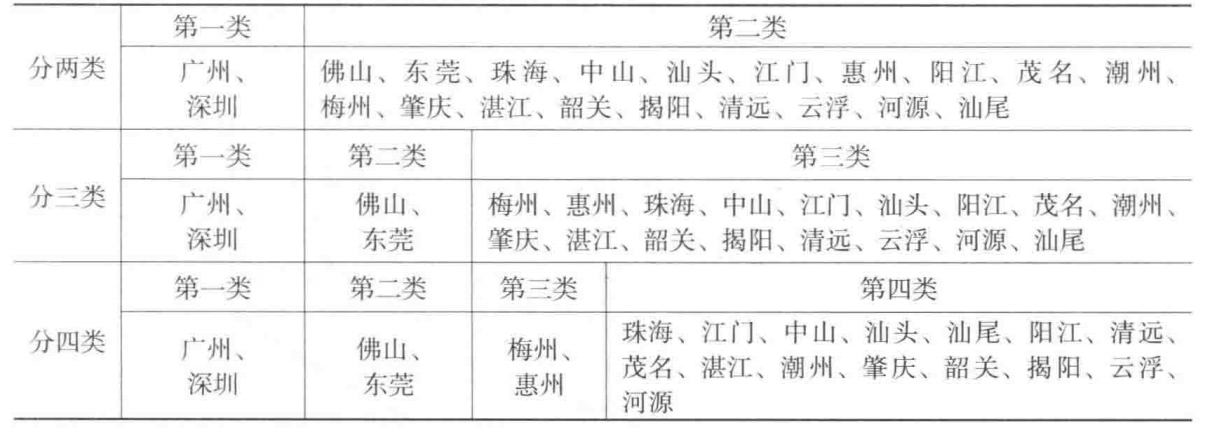
\includegraphics{./cluster_res.png}
\caption{image-2.png}
\end{figure}

从聚类结果可以看出,广东省电信业总量2003年排到了全国之首,但是各地区之间存在严重差异。对此,广东省政府应加快经济欠发达地区的电信建设,大力扩展山区电信市场,并采取扶持措施加强农村市场建设,促进广东省各地区电信业的协调发展。

    \hypertarget{ux4e3bux6210ux5206ux5206ux6790}{%
\subsection{主成分分析}\label{ux4e3bux6210ux5206ux5206ux6790}}

    \begin{tcolorbox}[breakable, size=fbox, boxrule=1pt, pad at break*=1mm,colback=cellbackground, colframe=cellborder]
\prompt{In}{incolor}{99}{\boxspacing}
\begin{Verbatim}[commandchars=\\\{\}]
\PY{n}{PC}\PY{o}{=}\PY{n+nf}{princomp}\PY{p}{(}\PY{n}{Case8}\PY{p}{,}\PY{n}{cor}\PY{o}{=}\PY{k+kc}{TRUE}\PY{p}{)}
\PY{n+nf}{summary}\PY{p}{(}\PY{n}{PC}\PY{p}{)}
\PY{n}{m}\PY{o}{=}\PY{l+m}{2}
\PY{n}{PC}\PY{o}{\PYZdl{}}\PY{n}{loadings}\PY{p}{[}\PY{l+m}{1}\PY{o}{:}\PY{n}{m}\PY{p}{]}
\PY{n+nf}{princomp.rank}\PY{p}{(}\PY{n}{PC}\PY{p}{,}\PY{n}{m}\PY{p}{)}\PY{c+c1}{\PYZsh{}主成分排名}
\PY{n+nf}{princomp.rank}\PY{p}{(}\PY{n}{PC}\PY{p}{,}\PY{n}{m}\PY{p}{,}\PY{n}{plot}\PY{o}{=}\PY{k+kc}{TRUE}\PY{p}{)}\PY{c+c1}{\PYZsh{}主成分作图}
\end{Verbatim}
\end{tcolorbox}

    
    \begin{Verbatim}[commandchars=\\\{\}]
Importance of components:
                          Comp.1    Comp.2     Comp.3      Comp.4      Comp.5
Standard deviation     2.2728344 1.2505211 0.44970504 0.227971879 0.120498454
Proportion of Variance 0.7379681 0.2234004 0.02889066 0.007424454 0.002074268
Cumulative Proportion  0.7379681 0.9613685 0.99025913 0.997683585 0.999757853
                             Comp.6       Comp.7
Standard deviation     0.0355324091 2.079601e-02
Proportion of Variance 0.0001803646 6.178203e-05
Cumulative Proportion  0.9999382180 1.000000e+00
    \end{Verbatim}

    
    \begin{enumerate*}
\item 0.435312447773798
\item 0.0973658680414553
\end{enumerate*}


    
    A matrix: 21 × 4 of type dbl
\begin{tabular}{r|llll}
  & Comp.1 & Comp.2 & PC & rank\\
\hline
	广州市 &  5.9067991 &  2.55970083 &  5.12900871 & 21\\
	珠海市 & -0.7333979 &  0.56847242 & -0.43087252 & 14\\
	汕头市 & -0.1481683 &  0.54948062 &  0.01394966 & 17\\
	深圳市 &  6.6864413 & -1.98309171 &  4.67183676 & 20\\
	佛山市 &  0.8354561 &  1.39474668 &  0.96542262 & 18\\
	韶关市 & -1.3050370 & -0.01633091 & -1.00557067 &  5\\
	河源市 & -1.3377517 & -0.42049544 & -1.12460200 &  2\\
	梅州市 & -0.7234574 & -2.38860477 & -1.11040019 &  3\\
	惠州市 &  0.3941757 & -2.85692104 & -0.36130606 & 15\\
	汕尾市 & -1.4768554 &  0.26395929 & -1.07232921 &  4\\
	东莞市 &  2.8592296 & -0.17266750 &  2.15468490 & 19\\
	中山市 & -0.3390609 &  1.06722611 & -0.01227143 & 16\\
	江门市 & -0.8325441 &  0.45906655 & -0.53240281 & 13\\
	阳江市 & -1.4745838 &  0.69356088 & -0.97075572 &  6\\
	湛江市 & -1.3101524 &  1.04963109 & -0.76179181 & 12\\
	茂名市 & -1.3822931 &  0.94188228 & -0.84220702 & 10\\
	肇庆市 & -0.9606084 & -0.70611954 & -0.90147089 &  9\\
	清远市 & -1.3041414 &  0.42559417 & -0.90218971 &  8\\
	潮州市 & -0.9043253 & -0.98540256 & -0.92316579 &  7\\
	揭阳市 & -1.0743640 & -0.03218726 & -0.83218556 & 11\\
	云浮市 & -1.3753608 & -0.41150020 & -1.15138126 &  1\\
\end{tabular}


    
    A matrix: 21 × 4 of type dbl
\begin{tabular}{r|llll}
  & Comp.1 & Comp.2 & PC & rank\\
\hline
	广州市 &  5.9067991 &  2.55970083 &  5.12900871 & 21\\
	珠海市 & -0.7333979 &  0.56847242 & -0.43087252 & 14\\
	汕头市 & -0.1481683 &  0.54948062 &  0.01394966 & 17\\
	深圳市 &  6.6864413 & -1.98309171 &  4.67183676 & 20\\
	佛山市 &  0.8354561 &  1.39474668 &  0.96542262 & 18\\
	韶关市 & -1.3050370 & -0.01633091 & -1.00557067 &  5\\
	河源市 & -1.3377517 & -0.42049544 & -1.12460200 &  2\\
	梅州市 & -0.7234574 & -2.38860477 & -1.11040019 &  3\\
	惠州市 &  0.3941757 & -2.85692104 & -0.36130606 & 15\\
	汕尾市 & -1.4768554 &  0.26395929 & -1.07232921 &  4\\
	东莞市 &  2.8592296 & -0.17266750 &  2.15468490 & 19\\
	中山市 & -0.3390609 &  1.06722611 & -0.01227143 & 16\\
	江门市 & -0.8325441 &  0.45906655 & -0.53240281 & 13\\
	阳江市 & -1.4745838 &  0.69356088 & -0.97075572 &  6\\
	湛江市 & -1.3101524 &  1.04963109 & -0.76179181 & 12\\
	茂名市 & -1.3822931 &  0.94188228 & -0.84220702 & 10\\
	肇庆市 & -0.9606084 & -0.70611954 & -0.90147089 &  9\\
	清远市 & -1.3041414 &  0.42559417 & -0.90218971 &  8\\
	潮州市 & -0.9043253 & -0.98540256 & -0.92316579 &  7\\
	揭阳市 & -1.0743640 & -0.03218726 & -0.83218556 & 11\\
	云浮市 & -1.3753608 & -0.41150020 & -1.15138126 &  1\\
\end{tabular}


    
    \begin{center}
    \adjustimage{max size={0.9\linewidth}{0.9\paperheight}}{output_42_4.png}
    \end{center}
    { \hspace*{\fill} \\}
    
    经过主成分分析,我们发现可以提取两个主成分,两个主成分的累计贡献率就达到了\(96.14\%\)

第一个主成分主要由\(X_1\)(电信业务总量)、\(X_4\)(国际互联网用户)、\(X_5\)(互联网用户使用时长)、\(X_6\)(长途电话通话量)、\(X_7\)(长途电话通话时长)决定,这5个指标是总量因素,说明一个城市的电信业规模和电信通信业务发展水平。

第二个主成分主要由\(X_2\)(每百人拥有固定电话数)、\(X_3\)(每百人拥有移动电话数)决定。这两个指标是平均量成分,反映了电信行业中的电话人均普及情况。

以主成分贡献率作为权数,计算城市电信业发展水平排名。公式为 \[
\frac{0.738PC_1 + 0.223PC_2}{0.738 + 0.223}
\]

从主成分得分图上可以清楚地看到,第一主成分和第二主成分得分最高的均为深圳,而稍有争议的排名是惠州、中山和茂名。惠州的第一主成分水平,即通信发展水平低于中山市,但是其第二主成分,即电话普及水平是远远超过中山的,而第二主成分的占比为\(22.34\%\),这也是不容忽视的。茂名市由于其互联网用户不够多而且人均电话普及量不够,两个主成分的得分都不高,而第二主成分尤其偏低,从而它的排名比较靠后。


    % Add a bibliography block to the postdoc
    
    
    
\end{document}
